\chapter{Background}

This section will explain the technical fundamentals which are necessary to understand the complete bachelor thesis.


\section{The CAN bus}

All communication performed and recorded in this thesis with an ECU is done via the Control Area Network bus (CAN).

Its specification is released in the ISO 11898. Each frame on this bus can transmit up to 8 bytes of payload and has an identifier with a length of either 11 or 29 bits, the former being more common. An identifier does not necessarily have to designate a physical device; it can also indicate one of several software modules of a device.
The maximum data rate is 1 Mbit/sec with a network length below 40\,m. The higher the length, the lower the possible data rate, as can be seen in \autoref{tab:can-speed}.

\begin{table}[htb]
    \centering
    \begin{tabular}{cc}
    \hline
    \textbf{Bus Length (m)} & \textbf{Signaling Rate (Mbps)}\\
    \hline
    40 & 1 \\
    100 & 0.5 \\
    200 & 0.25 \\
    500 & 0.10 \\
    1000 & 0.05 \\
    \hline
\end{tabular}
\caption{Suggested cable lengths for signaling rates of the CAN bus \cite{slla270}.}
\label{tab:can-speed}
\end{table}

\subsection{Advantages for the automotive domain}

This bus is robust because it uses two lines with differential signals for communication, i.e. when one line is driven high, the other is driven low. Thus, the receiver can reliably detect interferences by comparing these signals.

Moreover, CAN busses are using the bus network topology (as illustrated in \autoref{fig:with-without-can}). This reduces the number of wires compared to star topologies, resulting in lower weight, which is an important factor for manufacturers.

%with-without-can
\begin{figure}[htb]
    \centering
    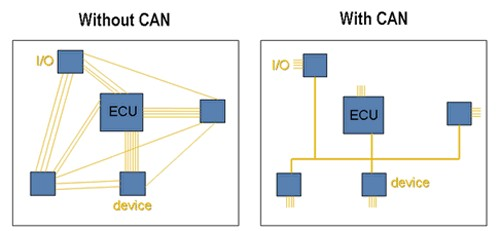
\includegraphics[width=0.7\textwidth]{with-without-can}
    \caption{CAN effect on decreasing the wire quantity \cite{Sharma2016}.}
    \label{fig:with-without-can}
\end{figure}

Last but not least, an important feature for the automotive application domain is the priority support. The lower the identifier, the higher the priority. Hence, if two ECUs transmit a CAN frame at exactly the same time, the frame with the lower identifier wins, the other one is discarded and will be retransmitted. This is called the Carrier Sense Multiple Access with Collision Detection (CSMA/CD) protocol \cite{Sharma2016}. For this reason, diagnostic CAN identifiers tend to have a high identifier \cite{Herrewegen2018}.

\subsection{Security vulnerabilities}

If you take this one step further, CAN is vulnerable to denial of service attacks. This attack can be performed by flooding the CAN bus with zero-identifier messages resulting in drops of legitimate frames \cite{Buttigieg2017}.

Furthermore, Buttigieg et al. \cite{Buttigieg2017} describe three more security issues of the CAN bus protocol in their paper \emph{Security Issues in Controller Area Networks in Automobiles}.
First, CAN frames do not contain any authentication information. An ECU receiving a message is not able to distinguish between a message from a legitimate ECU and a malicious one \cite{Buttigieg2017}. So, for example, if the state of an ECU is changed to a higher privileged state, all devices, including malicious ones, will have access to its newly unlocked services and information. Countermeasures exist in the form of performing authentication, but there is no satisfying solution yet, which fulfills cost-effectiveness, backward compatibility, support for vehicle repair and maintenance, sufficient implementation details, and acceptable overhead \cite{Bozdal2020}.
Also, originally, CAN bus networks lacked network segmentation, since each message is broadcasted and received by each node of the network \cite{Buttigieg2017}. Nowadays, car networks are usually divided into less and more critical segments by so-called Gateway ECUs \cite{Bozdal2020}. Despite the increase in the level of security, this makes it more difficult to maintain the system, which is associated with increased costs \cite{Bozdal2020}.
The final security vulnerability is the lack of data encryption \cite{Buttigieg2017}. Lightweight encryption systems could be implemented, but are limited by the short length of the data field (8 bytes) and the limited computing power of ECUs \cite{Bozdal2020}.

Since all countermeasures described in the previous paragraph are limited, Intrusion Detection Systems (IDS) are emerging, with the advantages of not having to change existing ECUs and not increasing bus traffic \cite{Bozdal2020}. A proof of concept of such systems was implemented by eMundo in preparation for the PetS3 project \cite{spahn2018}.

\subsection{Virtual CAN interfaces and using the can-utils}
\label{subsubsec:can-utils}

Virtual CAN interfaces can be used for simulations or simple tests. They are supported natively by Linux without additional actions.
To create a virtual CAN interface, only one command in a Linux shell is required (see line 1 of \autoref{lst:can-utils}).

\begin{listing}[H]
\begin{minted}
[frame=single,
framerule=0pt,
framesep=2mm,
baselinestretch=1.2,
bgcolor=VeryLightGray,
fontsize=\footnotesize,
linenos]{text}
sudo ip link add vcan0 type vcan
candump vcan0
candump -l vcan0
cansend vcan0 123#01.02
\end{minted}
\caption{How to use the can-utils.}
\label{lst:can-utils}
\end{listing}

The most common toolkit to work with the CAN bus are the can-utils \cite{can-utils}, which can usually be installed with the package manager of the distributions. The \mintinline{text}{candump} command (line 2) displays all messages of the CAN bus on interface \mintinline{text}{vcan0} in a terminal.

Adding the \mintinline{text}{-l} option changes the output to be more compact instead of human-readable and stores the received traffic in a \mintinline{text}{candump.log} file (line 3). All traffic recorded in this work was done with this command.

For sake of completeness, the \mintinline{text}{cansend} command (line 4) sends a CAN frame with the identifier \mintinline{text}{0x123} and the payload \mintinline{text}{0x01 0x02}:

\section{The ISO-TP transport protocol for CAN}

CAN frames have a payload size of 8 bytes. This is sufficient for most UDS requests, but not for many UDS responses. Thus, ISO-TP is used as the transport protocol on the CAN bus for UDS communication.

It is defined in ISO 15765-2 and increases the payload size to 4095 bytes per message. At least one byte of each CAN frame is then transport protocol information, indicating whether this segment contains the entire data or only a fragment of it, with more segments to come.

\section{The UDS protocol}
\label{sec:uds}

UDS stands for \emph{Unified diagnostic services} and is an application protocol defined in ISO 14229. This protocol defines the structures of request and response data for diagnostic purposes sent over an arbitrary data link \cite{iso14229}.

The reason for designing such a protocol was that cars developed in the last decades were more and more capable of self-diagnosis. A car repair shop only had to request this information from the car. But since there was no universal standard, car manufacturers tended to implement company-specific protocols for this purpose. UDS solves this by being an international standard and not company-specific. The \emph{Unified} in its name underlines this. 

%UDS stack
\begin{figure}[htb]
    \centering
    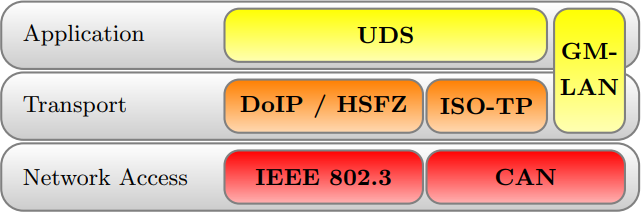
\includegraphics[width=0.7\textwidth]{uds-stack}
    \caption{The most common protocol stack for UDS \cite{Weiss2020}.}
    \label{fig:uds-stack}
\end{figure}

As shown in \autoref{fig:uds-stack}, the most common data links for the UDS protocol are Ethernet and the CAN bus. Others can and are used as well, explicitly stated in the UDS standard are FlexRay, K-Line and LIN.

\subsection{Services}
\label{subsubsec:uds-services}

UDS defines various services with different purposes. The ones used later in this thesis are explained here.

The \emph{RoutineControl} (RC) service enables the management of predefined routines on the ECU. They can be started, stopped or their results requested. Examples for routines are resetting or learning adaptive data, running a self-test or closing convertible roofs. It has two parameters, namely the desired action and the identifier of the routine.

Another service is called \emph{ReadDataByIdentifier} (RDBI). With this service, it is possible to retrieve one or more values of an ECU. This can be static information like the software version or dynamic values such as the current readings of sensors. It contains only the identifier of the requested data as a parameter.

The \emph{DiagnosticSessionControl} (DSC) service is used to enable different diagnostic states in the ECU, and the \emph{SecurityAccess} (SA) service to unlock restricted access to data or services. They are explained in more detail in the next section, as they affect the state of ECUs.

\subsection{States}
\label{subsec:states}

There is always exactly one global UDS state active for an ECU. It influences the behavior of the ECU and can be changed by sending specific requests. Just a few services are able to accomplish this. For example, sending a request to the SA or DSC service of an ECU may affect its state. Whether the ECU has actually changed the state can be easily determined by checking whether the sender received a positive or negative response from the ECU.

The default state is the active state after the ECU is switched on. Without an external request, it remains in this state. In the DSC service, each parameter value specifies a state. Thus, if the ECU designers integrated a state for $n$, the controller will respond positively to a DSC request to activate this state. It will now remain in this state until there has been no UDS communication for usually five seconds, then it will automatically return to the default state. If the ECU designers did not integrate such a state, it will answer with a negative response and remain in its current state.

The \emph{SecurityAccess} (SA) service uses the challenge–response authentication, in automotive terminology called seed-key protocol. The ECU sends a randomly generated value (the seed) to the client. Both devices generate a response (the key) based on the seed and the client sends its response to the ECU. If the keys match for the received and the generated response for the ECU, the client is authenticated (see \autoref{fig:key-seed}) \cite{iso14229}.

\begin{figure}[htb]
    \centering
    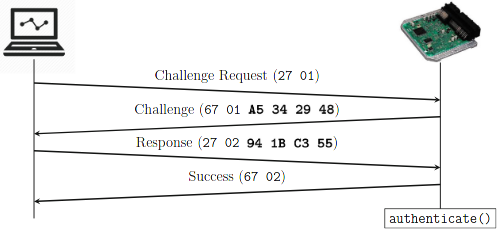
\includegraphics[width=0.7\textwidth]{key-seed}
    \caption{The challenge-response protocol \cite{Herrewegen2018}.}
    \label{fig:key-seed}
\end{figure}

\autoref{fig:ecu-state-behavior} illustrates the behavior of the ECU when a request is received for the DSC service and parameter value $n$. The state $n$ is considered as a state that can be further unlocked with the SA service.

\begin{figure}[htb]
    \centering
    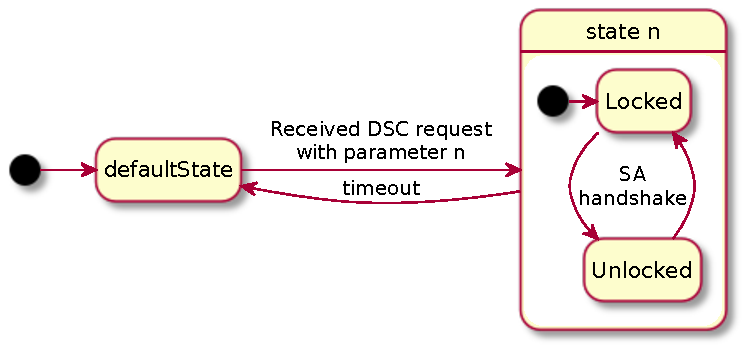
\includegraphics[width=0.7\textwidth]{uml/ecu-state-machine}
    \caption{Example of a state machine from an ECU for UDS.}
    \label{fig:ecu-state-behavior}
\end{figure}

\subsection{Data structure}

\begin{figure}[htb]
    \centering
    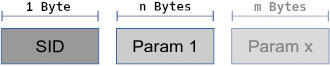
\includegraphics[width=0.5\textwidth]{uds-structure}
    \caption{The structure of UDS requests.}
    \label{fig:uds-structure}
\end{figure}

\autoref{fig:uds-structure} shows how UDS requests are structured. Each service is identified by a Service Identifier (SID). This identifier is the first byte in all UDS data. It must not be confused with the identifier of the CAN frame. Then at least one parameter follows. Most common is only one parameter, but services with multiple parameters exist too.
Negative responses have the SID \mintinline{text}{0x7f}.
For positive responses it is defined as \mintinline{text}{0x40} added to the SID. Thus, a request with SID \mintinline{text}{0x27} would be responded with \mintinline{text}{0x27 + 0x40 = 0x67} (see \autoref{fig:key-seed}).


\section{The UDS Scanner}
\label{sec:uds-scanner}

The UDS Scanner is a protocol scanner dedicated for the UDS protocol. It was implemented in the Scapy library, which is explained in more detail in \autoref{sec:scapy}.

\subsection{Purpose}

\begin{figure}[htb]
    \centering
    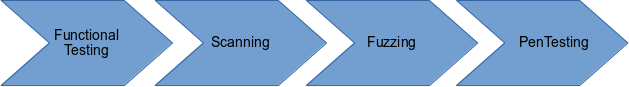
\includegraphics[width=0.8\textwidth]{automotive-security-testing-process}
    \caption{The Automotive Security Testing process.}
    \label{fig:automotive-security-testing-process}
\end{figure}

As \autoref{fig:automotive-security-testing-process} shows, the security testing process in the automotive domain contains a scanning step that aims to detect what services of a protocol are implemented and what information can be obtained in these services \cite{Bayer2015}. The UDS Scanner fulfills these tasks. It can also be used for fuzzing, even though scanning is its main use-case. The retrieved information answers the following questions:

\begin{itemize}
\item Which services are supported?
\item What information can be read with these services?
\item What control options does the ECU offer?
\item Which states does the ECU support and how does it behave in each case?
\end{itemize}


\subsection{Procedure}

The UDS Scanner starts with scanning each service for the default state of the ECU (see \autoref{subsec:states}). While doing so, it detects new states, which will be scanned subsequently. Therefore, as long as new states are found during an iteration, the scan continues. After each iteration, the ECU is reset to return to the default state. Then, the next state to be scanned is activated by sending a sequence of UDS requests, which is an edge of the UDS Scanner's internally built state machine. An ECU reset is usually done by switching off the ECU, waiting a few seconds, and switching it back on, although there is an ECU Reset service in the UDS protocol. However, its specification defines that the behavior is implementation-specific, so a power-based reset is the cleaner way.

\autoref{fig:uds-scanner-procedure} aims to make the procedure easier to understand.

\begin{figure}[htb]
    \centering
    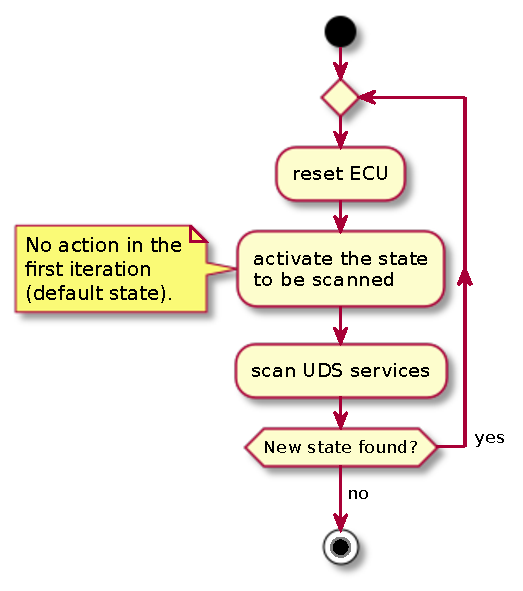
\includegraphics[width=0.5\textwidth]{uml/uds-scanner-procedure}
    \caption{Procedure of the UDS Scanner.}
    \label{fig:uds-scanner-procedure}
\end{figure}

\newpage

\section{The Scapy program}
\label{sec:scapy}

Scapy is the program in which the already mentioned protocols and the UDS Scanner of \autoref{sec:uds-scanner} were implemented.

\subsection{Overview}
The homepage of Scapy introduces itself with \cite{scapy}:
\begin{displayquote}
Scapy is a powerful interactive packet manipulation program. It is able to forge or decode packets of a wide number of protocols, send them on the wire, capture them, match requests and replies, and much more.
\end{displayquote}

Therefore, it fulfills the requirements of protocol scanners:
\begin{itemize}
    \item Receive and transmit packets
    \item Support for many physical layers and transport protocols
    \item Simple definition of packet structures
    \item Matching requests with their responses
\end{itemize}

It is used through a text-based user interface. This has the advantage of being lightweight, and working via ssh connections out-of-the-box. While being mainly a program, it can also be used as a library by importing the necessary classes and interfaces into an own program. Scapy is written in Python.

For the PetS3 project, many automotive features were added to Scapy. The diagnostic protocols GMLAN, UDS and OBD were implemented. As calibration protocols, the CAN Calibration Protocol (CCP) and its successor XCP were implemented. CAN and its transport protocol ISO-TP were also added to Scapy.

\subsection{UDS implementation in the Scapy library}
\label{subsec:uds-scapy}

One of the core classes in Scapy is the \mintinline{python}{Packet} class. All definitions of network layers, such as Ethernet, IP, TCP, CAN, UDS and so on, are defined in a class inheriting from it, regardless of the layer level.

Its most important member is the \mintinline{python}{fields_desc} list. It is a requirement for each layer to overwrite it. Its elements must inherit from the \mintinline{python}{Field} class. The chosen field classes define the structure of each header field.

\begin{listing}[H]
\begin{minted}
[frame=single,
framerule=0pt,
framesep=2mm,
baselinestretch=1.2,
bgcolor=VeryLightGray,
fontsize=\footnotesize,
linenos]
{python}
class UDS(Packet):
    services = {
            0x10: 'DiagnosticSessionControl',
            # [...]
            0x22: 'ReadDataByIdentifier',
            # [...]
            0x7f: 'NegativeResponse'}
    fields_desc = [
        XByteEnumField('service', 0, services)
    ]
\end{minted}
\caption{Implementation of the root class for UDS in Scapy.}
\label{lst:uds-implementation}
\end{listing}

The \mintinline{python}{UDS} class (see \autoref{lst:uds-implementation}) contains only an \mintinline{python}{XByteEnumField} field, representing the Service Identifier (SID). Field class names are composed of keywords.
\begin{samepage}
\begin{itemize}
    \item \mintinline{text}{X}: Represent its value as a hexadecimal value for the user.
    \item \mintinline{text}{Byte}: The field has 8 bits.
    \item \mintinline{text}{Enum}: The field maps machine-readable values to human-readable texts.
\end{itemize}
\end{samepage}

\mintinline{python}{X} and \mintinline{python}{Enum} only affect the representation of the field. The \mintinline{python}{Byte} keyword is the only one here that defines the actual structure of the field.

This field is given three parameters:

\begin{itemize}
    \item \mintinline{python}{'service'}: The name of the field.
    \item \mintinline{python}{0}: The default value of the field.
    \item \mintinline{python}{services}: The dictionary mapping from machine-readable values to human-readable texts.
\end{itemize}

The Scapy implementation starts a new class whenever the subsequent fields depend on a field value of the current layer. This is the case here, since the next fields depend on the SID. The service specific fields are defined in their own classes, for example the \mintinline{python}{UDS_DSC} class for the DSC service (see \autoref{lst:uds-dsc-implementation}).

\begin{listing}[H]
\begin{minted}
[frame=single,
framerule=0pt,
framesep=2mm,
baselinestretch=1.2,
bgcolor=VeryLightGray,
fontsize=\footnotesize,
linenos]
{python}
class UDS_DSC(Packet):
    diagnosticSessionTypes = {
            # [...]
            0x03: 'extendedDiagnosticSession',
            # [...]
    }
    fields_desc = [
        ByteEnumField('diagnosticSessionType', 0,  diagnosticSessionTypes)
    ]

bind_layers(UDS, UDS_DSC, service=0x10)
\end{minted}
\caption{Implementation of the DSC service in Scapy.}
\label{lst:uds-dsc-implementation}
\end{listing}

The \mintinline{python}{bind_layers} call (line 11 of \autoref{lst:uds-dsc-implementation}) tells Scapy the relationship between the classes \mintinline{python}{UDS} and \mintinline{python}{UDS_DSC}. This information is used by Scapy for building and interpreting data. Note that the keyword argument \mintinline{python}{service} has the same name as the field for the SID in the \mintinline{python}{UDS} class (see \autoref{lst:uds-implementation}).
Then, if UDS data is received with the SID \mintinline{text}{0x10}, it continues interpreting it with the field definitions of \mintinline{python}{UDS_DSC}. Vice versa, if \mintinline{python}{UDS_DSC} data is stacked on \mintinline{python}{UDS} data for building, its SID field is automatically set to \mintinline{text}{0x10}. Layers are stacked with the division operator of Python (see \autoref{lst:uds-dsc-stacking}). As can be seen, the SID of the UDS data is \mintinline{text}{0x10}, although it was never explicitly set. Scapy set it because of the previous binding.

\begin{listing}[H]
\begin{minted}
[frame=single,
framerule=0pt,
framesep=2mm,
baselinestretch=1.2,
bgcolor=VeryLightGray,
fontsize=\footnotesize,
linenos]
{python}
uds_data = UDS() / UDS_DSC(diagnosticSessionType=0x03)
bytes(uds_data) # prints: 0x10 0x03
\end{minted}
\caption{Stacking \mintinline{python}{UDS} and \mintinline{python}{UDS_DSC} to a complete UDS request.}
\label{lst:uds-dsc-stacking}
\end{listing}



\subsection{Transmit and receive UDS data via an ISO-TP socket}
\label{subsec:isotp}

As described in \autoref{sec:uds}, UDS mostly uses the ISO-TP protocol on the CAN bus for sending and transmitting data.
Scapy offers two ISO-TP sockets. A software and a native implementation. Both handle the ISO-TP communication themselves, for example segmentation and flow control.

The software version resolves the protocol communication in Scapy itself. Its advantage is the availability on all platforms.

The native socket uses an ISO-TP module for the Linux kernel. It uses the socket interface of Linux and brings all its advantages, such as asynchronous waiting for responses while the process is sleeping. Until including Linux kernel 5.9, this module had to be installed separately \cite{isotp-module}. Since kernel 5.10, it is part of the Linux mainline kernel \cite{isotp-commit}.

An ISO-TP socket contains a source and destination identifier. They have the same purpose as IP addresses. The source identifier (\mintinline{text}{sid}) is used for outgoing CAN frames, and the destination identifier (\mintinline{text}{did}) for incoming frames. In other words, the \mintinline{text}{sid} must contain the identifier to which the ECU expects requests, and the \mintinline{text}{did} must contain the identifier with which it responds. They must be known to be able to send requests to ECUs and receive their responses. The \mintinline{python}{basecls} argument tells the socket how to interpret incoming data.

The usage of the native implementation is presented by the following code snippet:

\begin{listing}[H]
\begin{minted}
[frame=single,
framerule=0pt,
framesep=2mm,
baselinestretch=1.2,
bgcolor=VeryLightGray,
fontsize=\footnotesize,
linenos]
{python}
from scapy.contrib.isotp import ISOTPNativeSocket as ISOTPSocket
socket = ISOTPSocket('vcan0', sid=0x123, did=0x456, basecls=UDS)
uds_data = UDS() / UDS_DSC(diagnosticSessionType=0x03)
# sr1 stands for: send and receive one response
response = socket.sr1(uds_data)
bytes(response) # prints: 50 00 32 01 f4 (hex)
\end{minted}
\caption{Sending a UDS request and receive its response with an ISO-TP socket.}
\label{lst:send-packet-isotp}
\end{listing}

The resulting frame and its response by the ECU from \autoref{lst:send-packet-isotp} can be observed with the \mintinline{text}{candump} program shown in \autoref{subsubsec:can-utils}. 

\begin{samepage}
\begin{minted}{text}
    $ candump vcan0
    vcan0  123   [3]  02 10 03
    vcan0  456   [7]  06 50 03 00 32 01 f4
\end{minted}
\end{samepage}

The request is explained step by step in the following list:

\begin{itemize}
    \item \mintinline{text}{0x123}: The CAN identifier.
    \item \mintinline{text}{[3]}: The length of the CAN payload.
    \item \mintinline{text}{0x02}: ISO-TP data showing the length of the layer 7 (UDS) payload.
    \item \mintinline{text}{0x10}: The SID of the DSC service.
    \item \mintinline{text}{0x03}: The parameter for the DSC service.
\end{itemize}
